\subsection{Advanced Encryption Standard (AES)}

Dado que el tamaño de bloque y la longitud de la llave de \acrshort{gl:des}
se volvieron muy pequeños para resistir los embates del progreso
de la tecnología, el \acrshort{gl:nist} comenzó la búsqueda de un nuevo cifrado
estándar en 1997; este cifrado debía tener un tamaño de bloque de,
al menos, 128 bits y soportar tres tamaños de llave: 128, 192 y 256 bits.

Después de pasar por un proceso de selección, la propuesta Rijndael fue
seleccionada. Se le hicieron algunas modificaciones, pues Rijndael soporta
combinaciones de llaves y bloques de longitud 128, 169, 192, 224 y 256;
mientras que \acrshort{gl:aes} tiene fijo el tamaño de bloque y solo utiliza
los tres tamaños de llave mencionados anteriormente. Dependiendo del tamaño 
de la llave, se tiene el número de \glspl{gl:ronda}: 10 para las de 128 bits,
12 para las de 192 y 14 para las de 256.

El cifrado requiere de una matriz de $4 \times 4$ denominada matriz de
estado.

\begin{pseudocodigo}[caption={AES, cifrado.}, label={aes:1}]
  entrada:    128 bits de texto en claro $M$; llave de $n$ bits $K$.
  salida:     bloque de texto cifrado de 64 bits $C = c_1 \dots c_{64}$.
  inicio
    Obtener las subllaves de 128 bits necesarias: una para cada ronda y una extra.
    Iniciar matriz de estado con el bloque en claro.
    Realizar $AddRoundKey(matriz\_estado, k_0)$
    para_todo $i$ desde 1 hasta $num\_rondas-1$:
      $SubBytes(matriz\_estado)$
      $ShiftRows(matriz\_estado)$
      $MixColumns(matriz\_estado)$
      $AddRoundKey(matriz\_estado, k_i)$
    fin
    $SubBytes(matriz\_estado)$
    $ShiftRows(matriz\_estado)$
    $MixColumns(matriz\_estado)$
    $AddRoundKey(matriz\_estado, k_{num\_rondas})$
    regresa $matriz\_estado$
  fin
\end{pseudocodigo}

Como todos los pasos realizados en las \glspl{gl:ronda} son invertibles, el
proceso de descifrado consiste en aplicar las funciones inversas a
$SubBytes$, $ShiftRows$, $MixColumns$ y $AddRoundKey$ en el orden
opuesto.

\subsubsection{SubBytes}
Esta es la única transformación no lineal de Rijndael. Sustituye
los bytes de la matriz de estado byte a byte al aplicar la función
$S_{RD}$ a cada elemento de la matriz. La función $S_{RD}$ es también
conocida como Caja-S y no depende de la llave. La misma caja es utilizada
para los bytes en todas las posiciones.

\begin{figure}[H]
  \begin{center}
    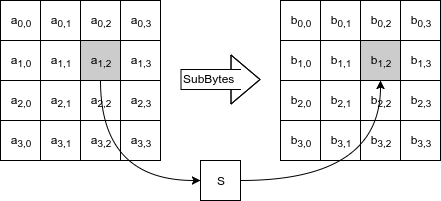
\includegraphics[width=0.6\linewidth]
      {contenidos/antecedentes/bloques/diagramas/subBytes}
     \caption{Diagrama de la operación $SubBytes$.}
   \end{center}
\end{figure}

\subsubsection{ShiftRows}
Esta transformación hace un corrimiento cíclico hacia la izquierda de las
filas de la matriz de estado. Los desplazamientos son distintos para cada
fila y dependen de la longitud del bloque ($N_b$).

\begin{figure}[H]
  \begin{center}
    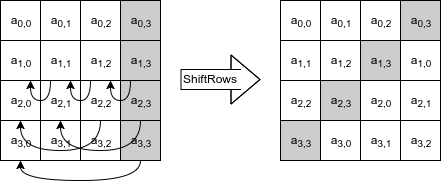
\includegraphics[width=0.6\linewidth]
      {contenidos/antecedentes/bloques/diagramas/shiftRows}
     \caption{Diagrama de la operación $ShiftRows$.}
   \end{center}
\end{figure}

\subsubsection{MixColumns}
Esta transformación opera en cada columna de la matriz de estado
independientemente. Se considera una columna $a = (a_0, a_1, a_2, a_3)$
como el polinomio $a(X) = a_3X^3 + a_2X^2 + a_1X + a_0$.
Entonces este paso transforma una columna $a$ al multiplicarla con el
siguiente polinomio fijo:
\begin{equation}
  \label{cifrado_aes_poli}
  c(X) = 03X^3 + 01X^2 + 01X+ 02
\end{equation}
y se toma el residuo del producto módulo $X^4+1$:
\begin{equation}
  \label{cifrado_aes_mix}
  a(X) \mapsto a(X) \cdotp c(X) \mod (X^4+1)
\end{equation}

\begin{figure}[H]
  \begin{center}
    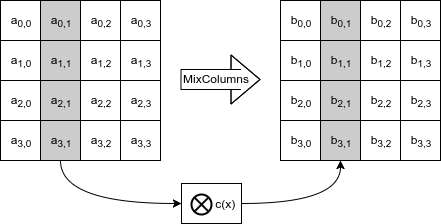
\includegraphics[width=0.6\linewidth]
      {contenidos/antecedentes/bloques/diagramas/mixColumns}
     \caption{Diagrama de la operación $MixColumns$.}
   \end{center}
\end{figure}

\subsubsection{AddRoundKey}
Esta es la única operación que depende de la llave secreta $k$. Añade una
llave de ronda para intervenir en el resultado de la matriz de estado.
Las llaves de ronda son derivadas de la llave secreta $k$ al aplicar el
algoritmo de generación de llaves. Las llaves de ronda tienen la misma
longitud que los bloques. Esta operación es simplemente una operación
$XOR$ bit a bit de la matriz de estado con la llave de ronda en turno.
Para obtener el nuevo valor de la matriz de estado se realiza lo
siguiente:
\begin{equation}
  \label{cifrado_aes_addkey}
  (matriz\_estado, k_i) \mapsto matriz\_estado \oplus k_i
\end{equation}

Como se tiene una matriz\_estado, la llave de ronda ($k_i$) también
es representada como una matriz de bytes con 4 columnas y $N_b$ columnas.
Cada una de las $N_b$ palabras de la llave de ronda corresponde a una
columna. Entonces se realiza la operación $XOR$ bit a bit sobre las
entradas correspondientes de la matriz de estado y la matriz de la llave
de ronda.

\begin{figure}[H]
  \begin{center}
    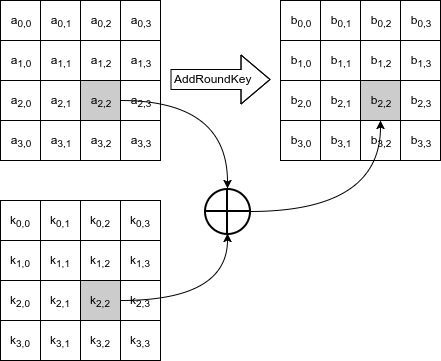
\includegraphics[width=0.6\linewidth]
      {contenidos/antecedentes/bloques/diagramas/addRoundKey}
     \caption{Diagrama de la operación $AddRoundKey$.}
   \end{center}
\end{figure}

Esta operación, claro está, es invertible: basta con aplicar la misma
operación con la misma llave para revertir el efecto.
